%%%%%%%%%%%%%%%%%%%%%%%%%%%%%%%%%%%%%%%%%%%%%%%%%%%%%%%%%%%%%%%%%%%%%%
% LaTeX Example: Project Report
%
% Source: http://www.howtotex.com
%
% Feel free to distribute this example, but please keep the referral
% to howtotex.com
% Date: March 2011 
% 
%%%%%%%%%%%%%%%%%%%%%%%%%%%%%%%%%%%%%%%%%%%%%%%%%%%%%%%%%%%%%%%%%%%%%%
% How to use writeLaTeX: 
%
% You edit the source code here on the left, and the preview on the
% right shows you the result within a few seconds.
%
% Bookmark this page and share the URL with your co-authors. They can
% edit at the same time!
%
% You can upload figures, bibliographies, custom classes and
% styles using the files menu.
%
% If you're new to LaTeX, the wikibook is a great place to start:
% http://en.wikibooks.org/wiki/LaTeX
%
%%%%%%%%%%%%%%%%%%%%%%%%%%%%%%%%%%%%%%%%%%%%%%%%%%%%%%%%%%%%%%%%%%%%%%
% Edit the title below to update the display in My Documents
%\title{Project Report}
%
%%% Preamble
\documentclass[10pt,letterpaper,oneside]{article}
\usepackage[T1]{fontenc}
\usepackage{fourier}
\usepackage{algorithm}
\usepackage{algorithmic}
\usepackage{tikz}
\usetikzlibrary{automata,positioning}
\usepackage{amsmath}
\usepackage{tikz}
\usetikzlibrary{arrows,automata}
\usepackage{listings}
\usepackage[margin=1in]{geometry}
\usepackage{hyperref}
%\hypersetup{pdftex,colorlinks=true,allcolors=blue}
\usepackage{hypcap}
\usepackage[english]{babel}															% English language/hyphenation
\usepackage[protrusion=true,expansion=true]{microtype}	
\usepackage{amsmath,amsfonts,amsthm} % Math packages
\usepackage[utf8]{inputenc}
% \usepackage[pdftex]{graphicx}
% \graphicspath{ {./images/} }
\usepackage{xurl}
\usepackage[acronym, toc]{glossaries}


%%% Custom sectioning
\usepackage{sectsty}
\allsectionsfont{\normalfont\scshape}


%%% Custom headers/footers (fancyhdr package)
\usepackage{fancyhdr}
\pagestyle{fancyplain}
\fancyhead{}											% No page header
\fancyfoot[L]{Hansen \& Karnani}											% Empty 
\fancyfoot[C]{\LaTeX}											% Empty
\fancyfoot[R]{\thepage}									% Pagenumbering
\renewcommand{\headrulewidth}{0pt}			% Remove header underlines
\renewcommand{\footrulewidth}{0pt}				% Remove footer underlines
\setlength{\headheight}{13.6pt}


%%% Equation and float numbering
\numberwithin{equation}{section}		% Equationnumbering: section.eq#
\numberwithin{figure}{section}			% Figurenumbering: section.fig#
\numberwithin{table}{section}				% Tablenumbering: section.tab#


%%% Maketitle metadata
\newcommand{\horrule}[1]{\rule{\linewidth}{#1}} 	% Horizontal rule

\title{
		%\vspace{-1in} 	
		\usefont{OT1}{bch}{b}{n}
		\huge CS 432 Final Project Documentation \\
		\horrule{2pt} \\[0.5cm]
}
\author{
		\normalfont 
		\normalsize
		Stephen Hansen, Kevin Karnani\\
        \normalsize
        \today\\
        \normalsize
        CS 432
} \date{}

\makeglossaries
\newglossaryentry{API}
{
        name=API,
        description={An application programming interface (API) is a set of programming directions that enables developers to access and include another web app’s information into their own application}
}
\newglossaryentry{database}
{
        name=database,
        description={A database (DB) contains information that is organized in such a way that it can be easily accessed, managed, and manipulated}
}
\newacronym{api}{API}{Application Programming Interface}
\newacronym{db}{DB}{Database}
\newacronym{sql}{SQL}{Structured Query Language}


%%% Begin document
\begin{document}
\maketitle\thispagestyle{empty}
\tableofcontents
\newpage
\clearpage
\setcounter{page}{1}
\section{Introduction}

For our final project, we wanted to create an interactive 3D world that took inspiration from the vaporwave art style. Vaporwave was a genre of music and art style that became popular in the early 2010s on the internet, but is now considered a dead genre. Album and single covers for vaporwave music traditionally had a trippy 80s arcade aesthetic, inspired by games such as Sega's Out Run. Some traditional aspects of vaporwave art include a grid plane, a large sun, Greek architecture, palm trees, Japanese characters, dolphins, and early 90s computer programs. Some have considered vaporwave art to be a parody of ``nostalgic'' art.

\noindent
\begin{center}
\textbf{Examples of Vaporwave}

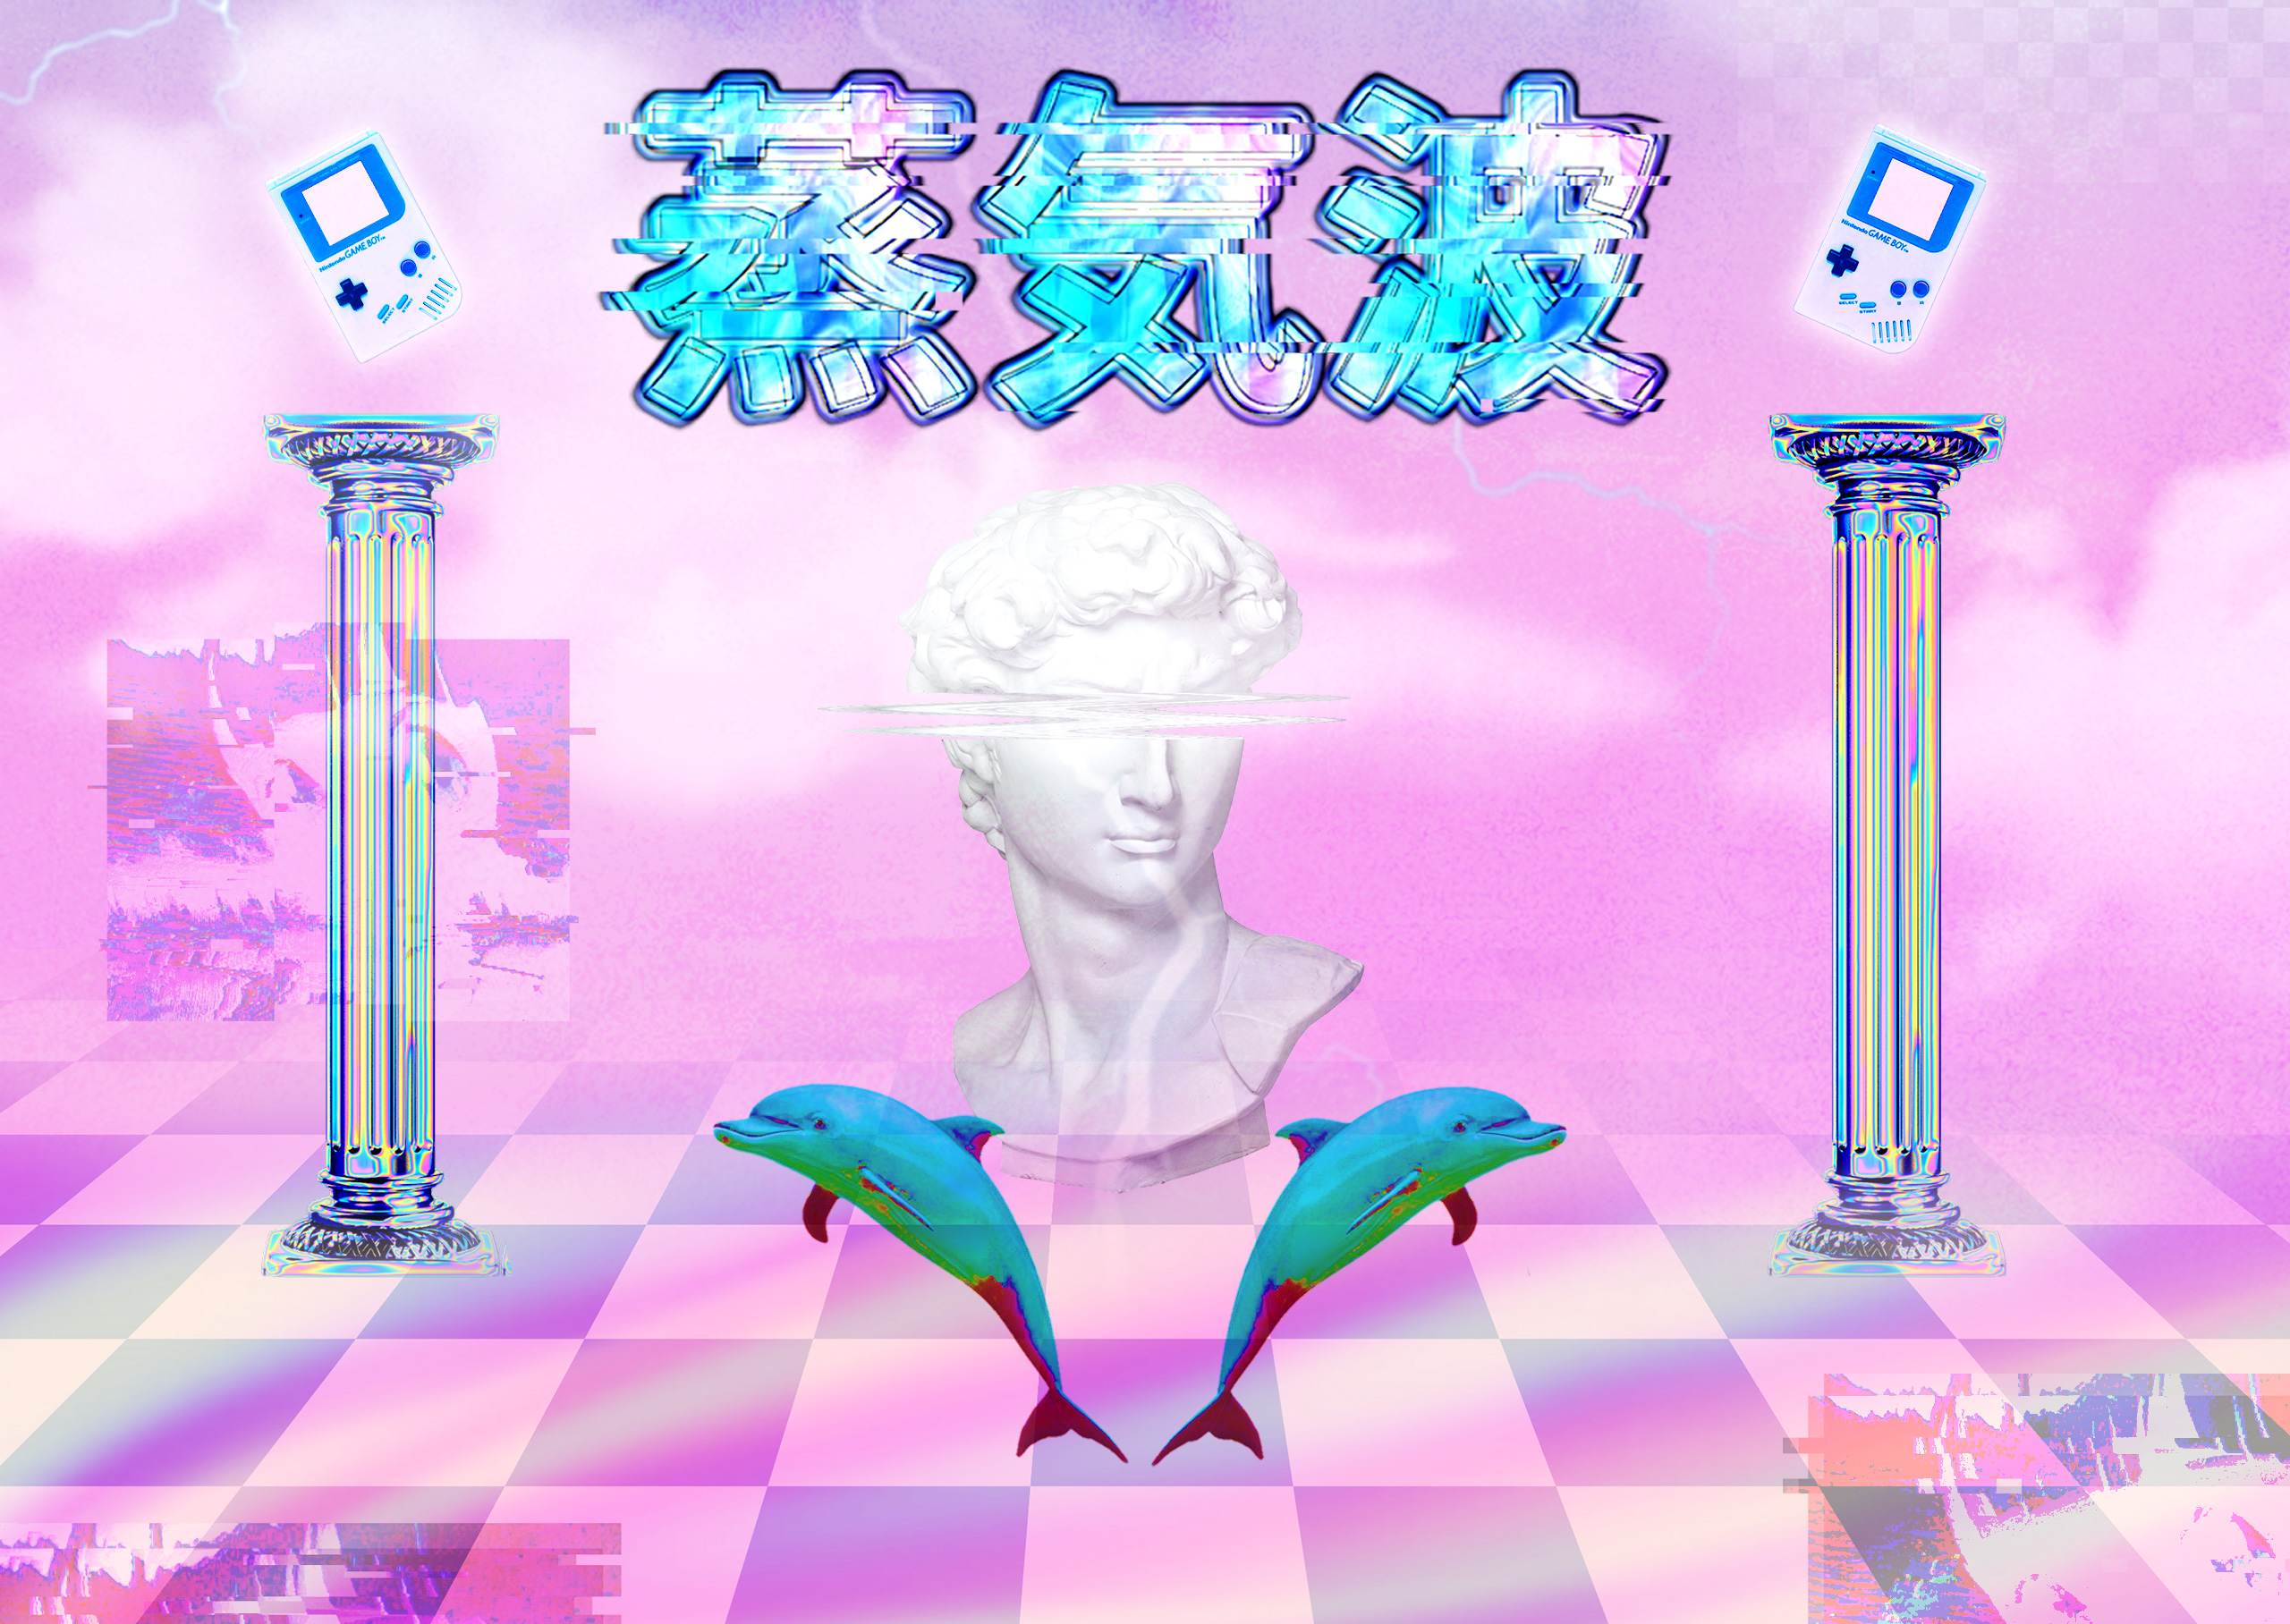
\includegraphics[width=0.3\textwidth]{vaporwave2.jpg}
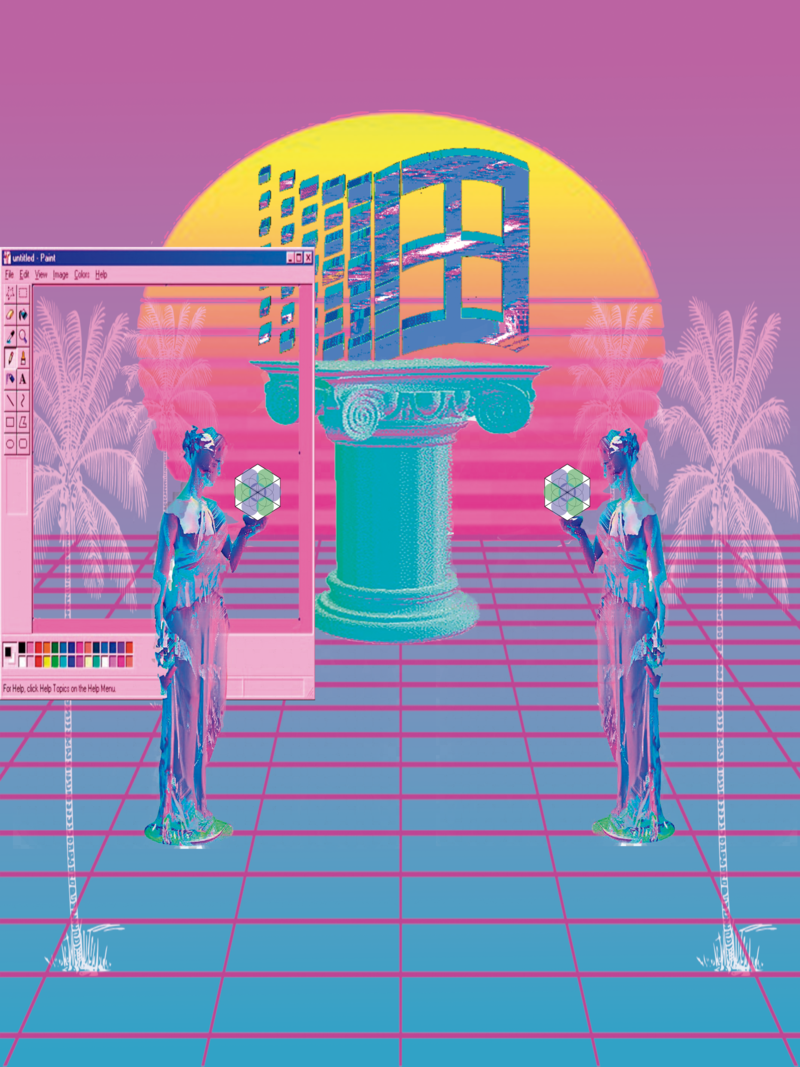
\includegraphics[width=0.3\textwidth]{vaporwave1.png}
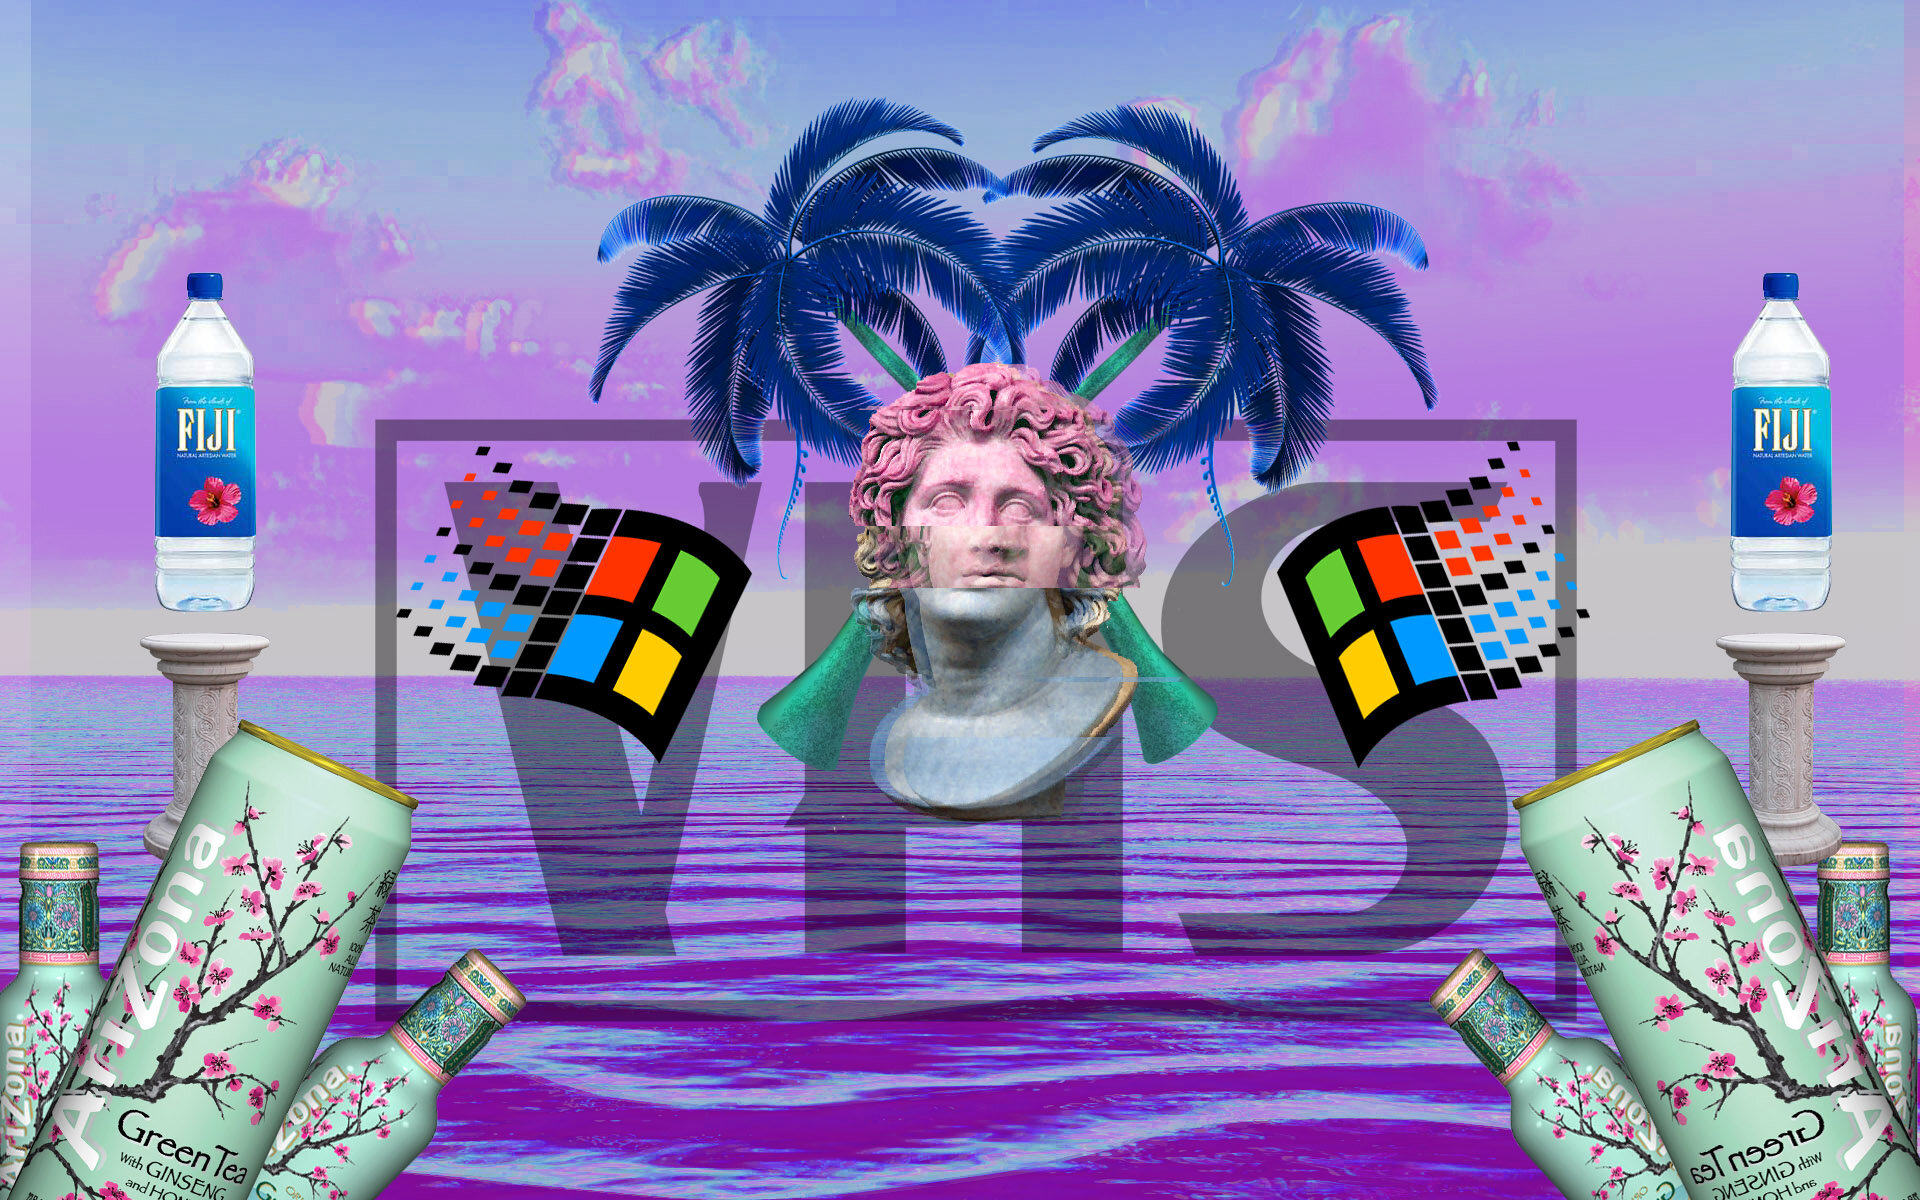
\includegraphics[width=0.3\textwidth]{vaporwave3.jpg}
\end{center}

Our project incorporates many aspects of the vaporwave genre. As the centerpiece to our 3D world, we have recreated the famous Greek Parthenon complete with a large statue inside. We have included elements such as palm trees and dolphins by creating our own .OBJ file loader module. There are two cameras to explore the world with; one camera is a flying free-cam that you can use to view the world from anywhere, the other camera is a first-person camera where you drive a reflective Tesla CyberTruck throughout the world. With this world, we have also implemented support for picking, dynamically generated objects, animated objects, reflection, shadows, and particle systems. The end result is a world that closely resembles aspects of the vaporwave genre shown here, with interactive components, and screenshots of the world would make for good vaporwave album covers.

\newpage
\section{Users Guide}

For our project, there are two cameras that you may switch between: a free-flying camera and a truck first-person camera. By default you start with the free-flying camera. Here is the default view of the scene. Note that some elements, like palm trees, Fiji water bottles, rain, and dolphins, are randomly generated every time you load the webpage. So your default view may not look exactly like this.
\begin{center}
    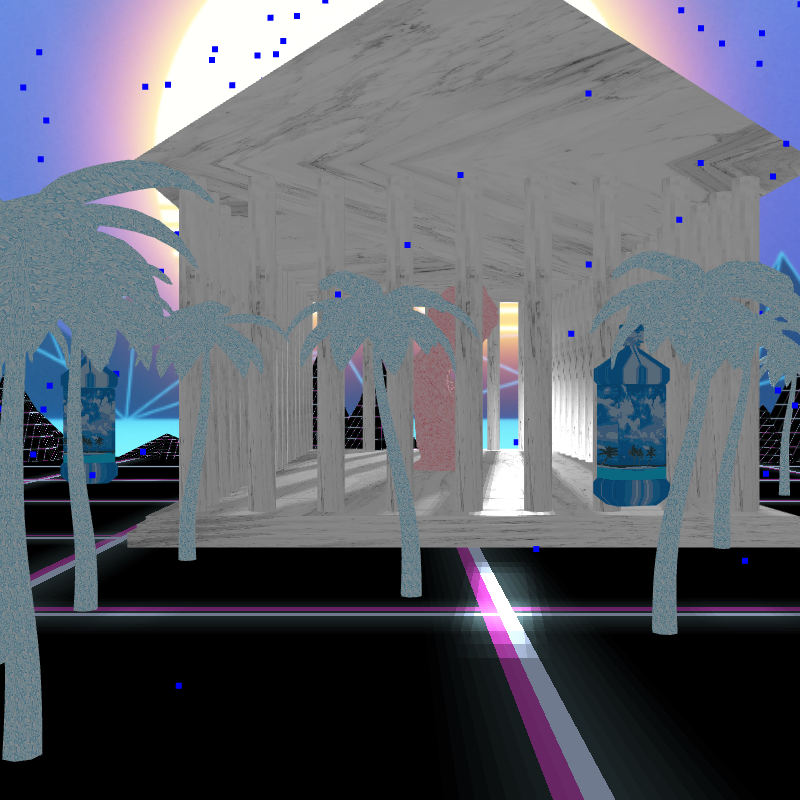
\includegraphics[width=0.5\textwidth]{start.png}
    
    The default view of the scene.
\end{center}

The default camera can move around using the forward and backward arrow keys to move the camera forward and backward. The left and right arrow keys respectively move the camera left and right. Use Shift and the Z key to roll counterclockwise and just the Z key (no shift) to roll clockwise. Shift and the X key can be used to pitch up and just the X key (no shift) can be used to pitch down. Finally, shift and the C key can be used to yaw counterclockwise, and just the C key (no shift) can be used to yaw clockwise.

The default scene has as a centerpiece a Parthenon with a rose quartz statue inside. There are many crystal palm trees randomly placed around the Parthenon. There are also floating animated Fiji water bottles located throughout the scene. The edges of the scene feature jagged mountains. The skybox follows the vaporwave theme being a large rising sun with mountains in the background. There is a reflective Tesla CyberTruck next to the Parthenon, and there is a particle system being used to simulate rain everywhere (except inside the Parthenon). There are two light sources: the first light source is the sun pictured in the skybox as a directional light source which gives off shadows. The second light source is a spotlight coming off the headlights of the CyberTruck.

Presented below are some pictures of this scene using the free-flying camera.

\begin{center}
    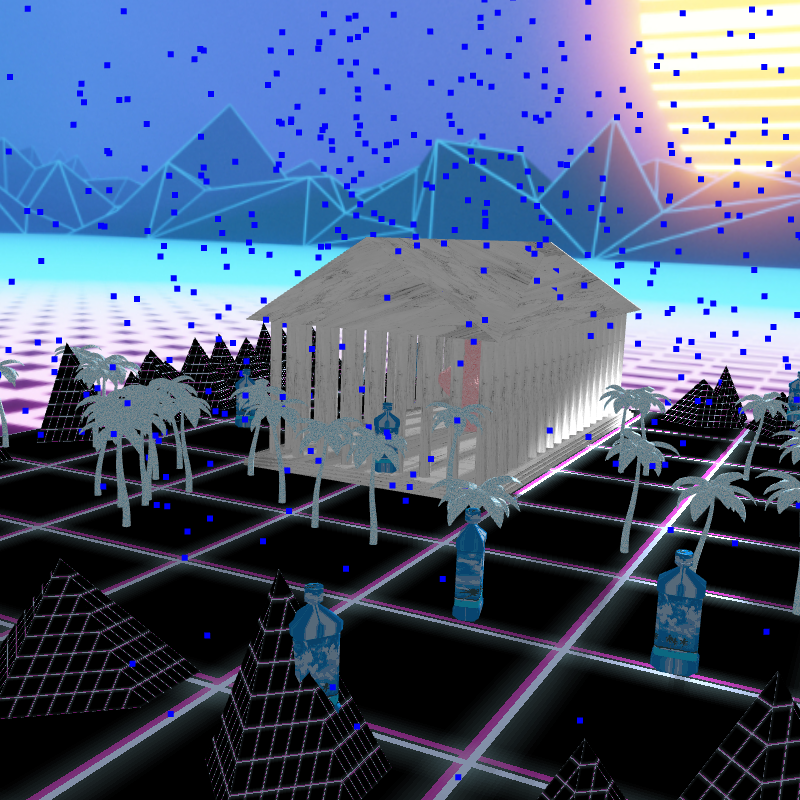
\includegraphics[width=0.5\textwidth]{scene1.png}
    
    The entire scene landscape.
    
    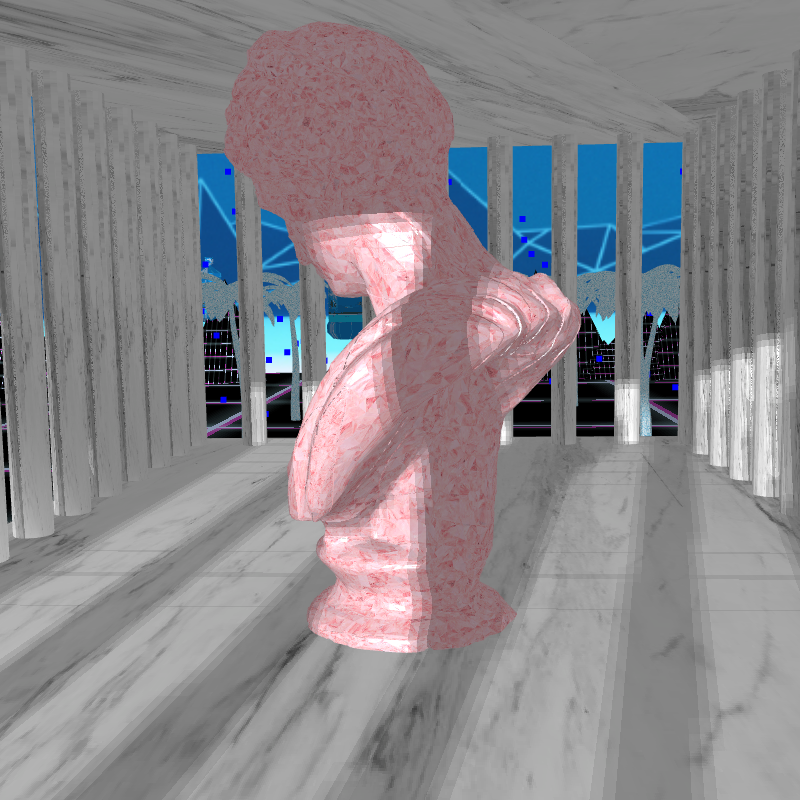
\includegraphics[width=0.5\textwidth]{scene2.png}
    
    Inside the Parthenon.
    
    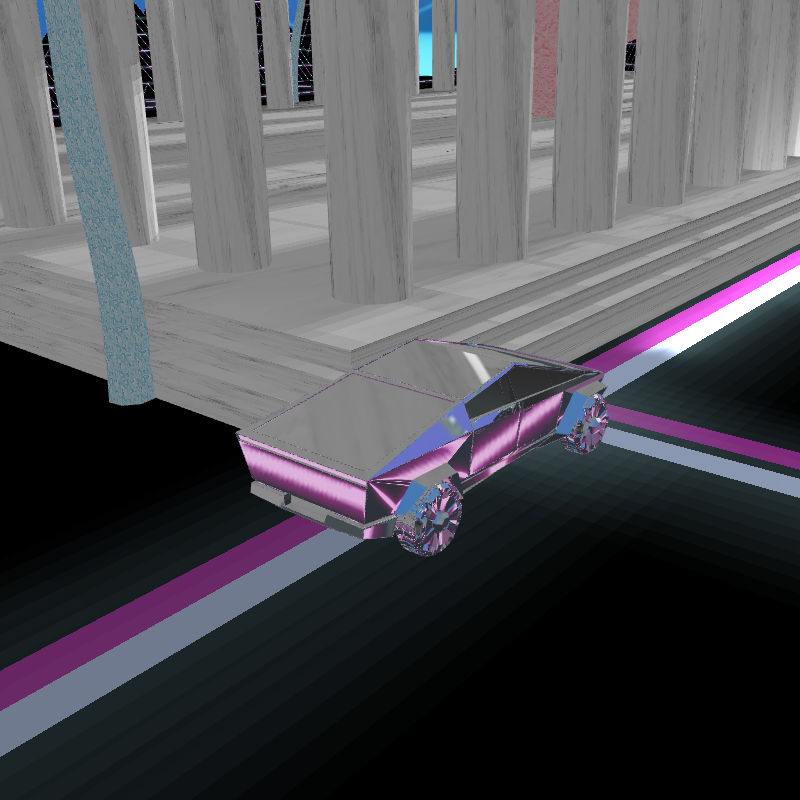
\includegraphics[width=0.5\textwidth]{scene3.png}
    
    The reflective CyberTruck.
    
    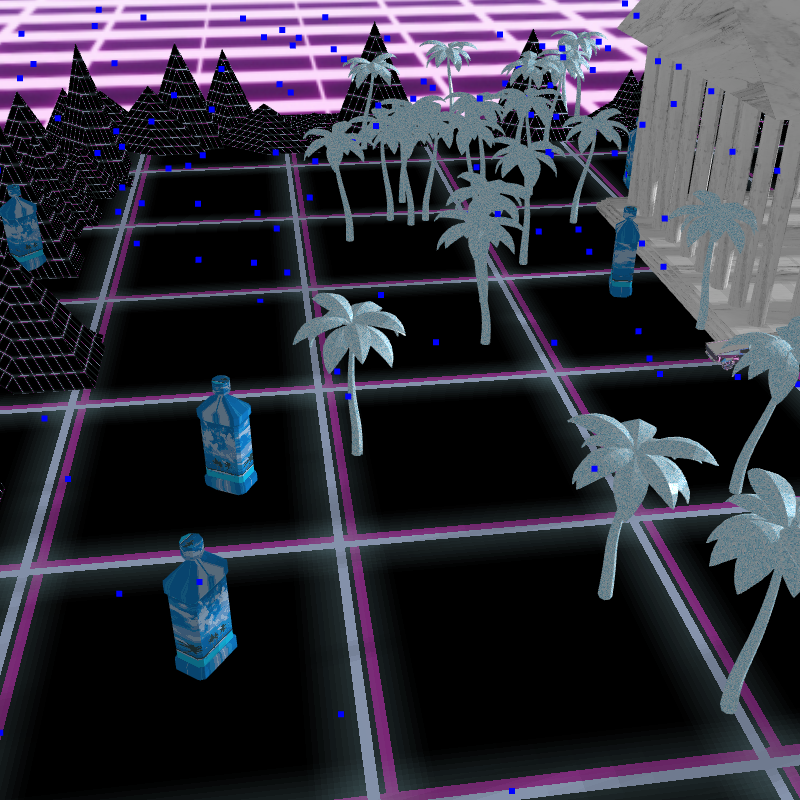
\includegraphics[width=0.5\textwidth]{scene4.png}
    
    Palm Trees, Fiji water bottles, and mountains - distinct elements of vaporwave artwork.
\end{center}

To switch between cameras, press the spacebar. The other camera provided is a first-person camera where you control the CyberTruck. The controls for the CyberTruck camera are different. Press the forward and backward keys to move the truck forward and backward. The left and right keys are used to turn the truck left and right. While driving the truck, there is an animated oil filter and CRT filter applied to the view. This makes the view interesting and simulates rain falling on the truck's window.

Presented below are some pictures of this scene using the truck camera.

\begin{center}
    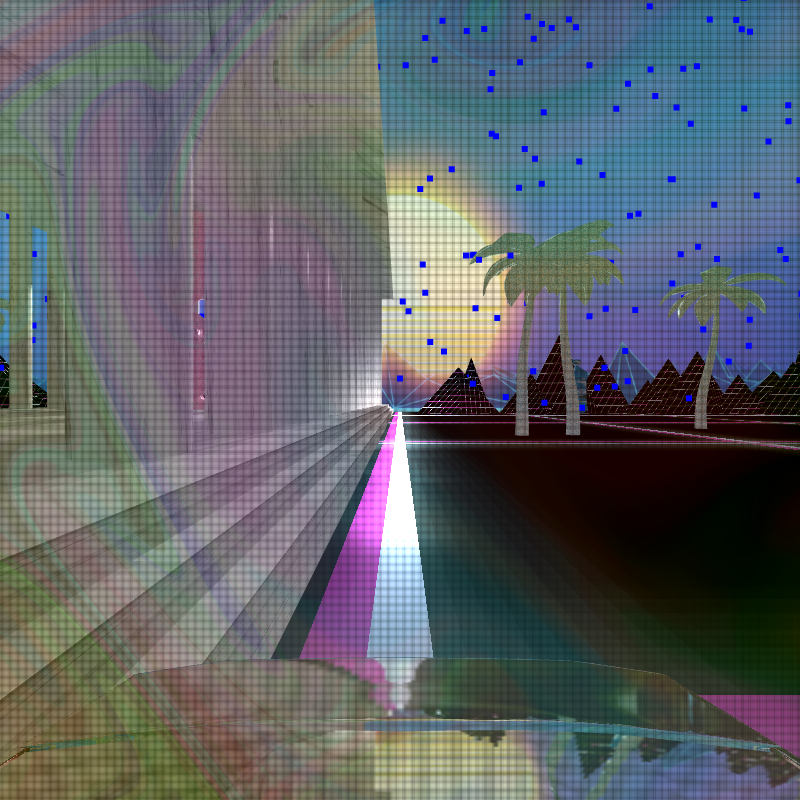
\includegraphics[width=0.5\textwidth]{truck1.png}
    
    The default view of the truck.
    
    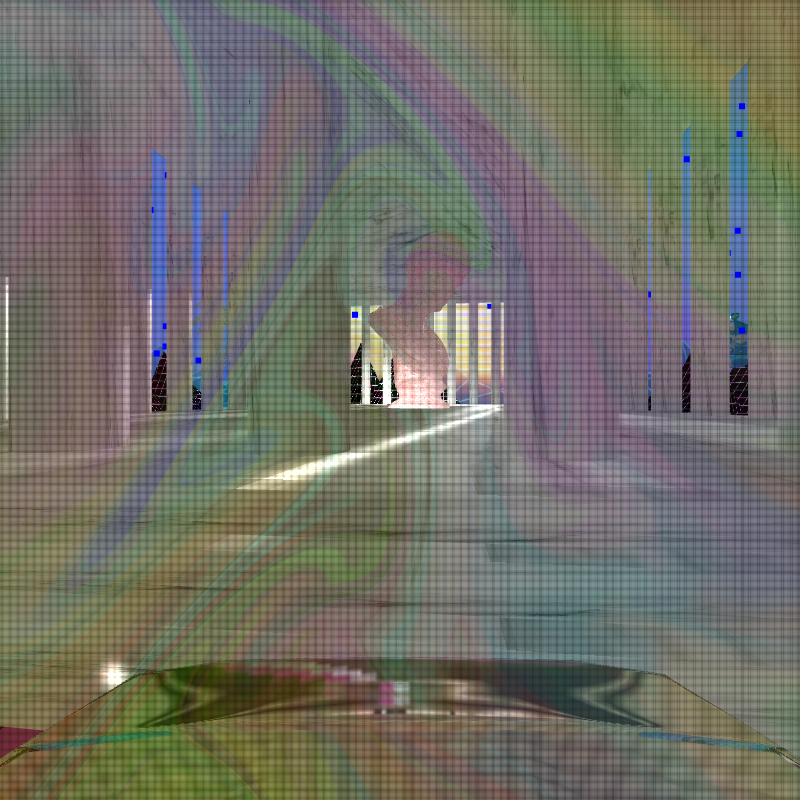
\includegraphics[width=0.5\textwidth]{truck2.png}
    
    Shining the headlights at the statue inside the Parthenon.
    
    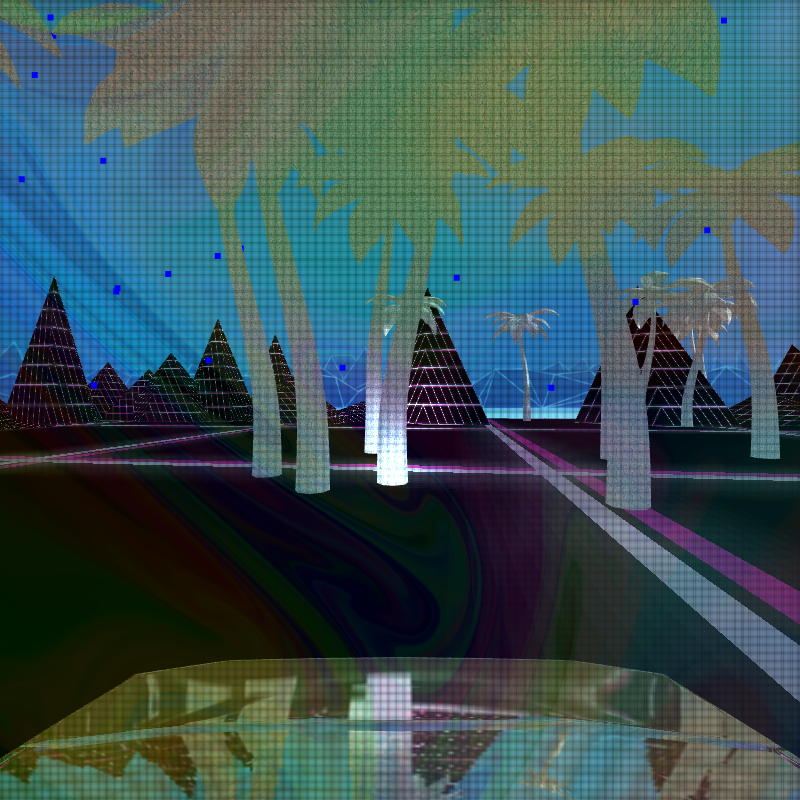
\includegraphics[width=0.5\textwidth]{truck3.png}
    
    Pointing our headlights towards some palm trees.
    
    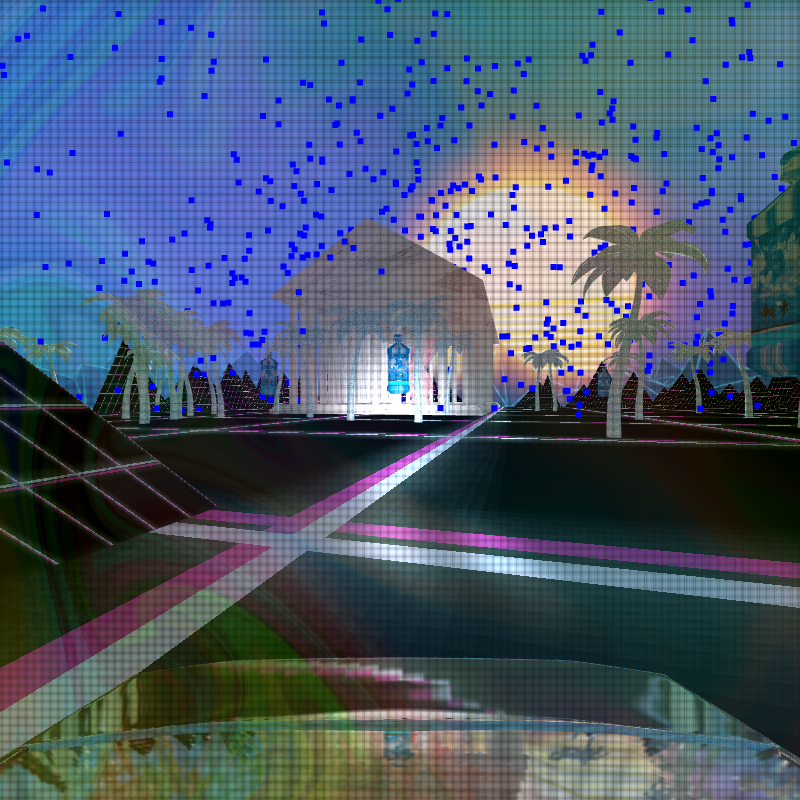
\includegraphics[width=0.5\textwidth]{truck4.png}
    
    Looking at the Parthenon from far away.
\end{center}

You can also switch back to the free-flying camera (press spacebar) to see that the truck has indeed moved location from where you last left it.

\begin{center}
    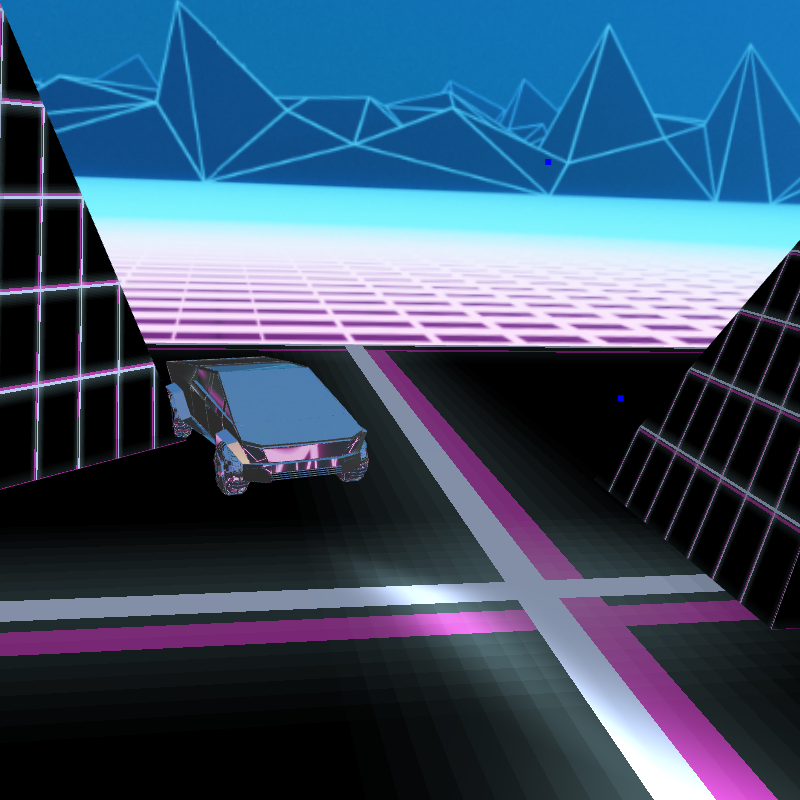
\includegraphics[width=0.5\textwidth]{moved.png}
    
    In free-flying camera mode; the truck is where we last left it.
\end{center}

In addition you may dynamically create a dolphin which leaps over the Parthenon. To create a new dolphin, press the ``s'' key. Every time you press this key, a new dolphin is randomly added to the scene. The dolphin will leap over the Parthenon to the other side of the map, where it will then be removed from scene. You may create as many dolphins as you want at any given time.

\begin{center}
    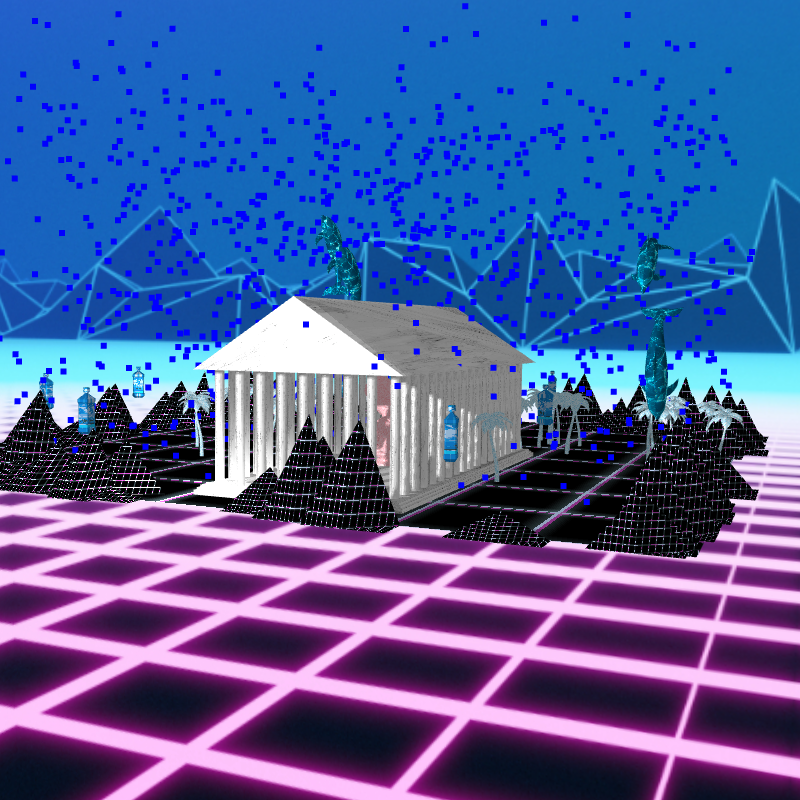
\includegraphics[width=0.5\textwidth]{dolphins.png}
    
    Four dolphins gracefully leap over the Parthenon.
\end{center}

% Picking

In addition we have implemented picking. Some objects are interactable when clicked on. If you click on a Fiji water bottle, it will grow and shrink in size. If you click on the statue inside the Parthenon, it will spin in a circle.

\begin{center}
    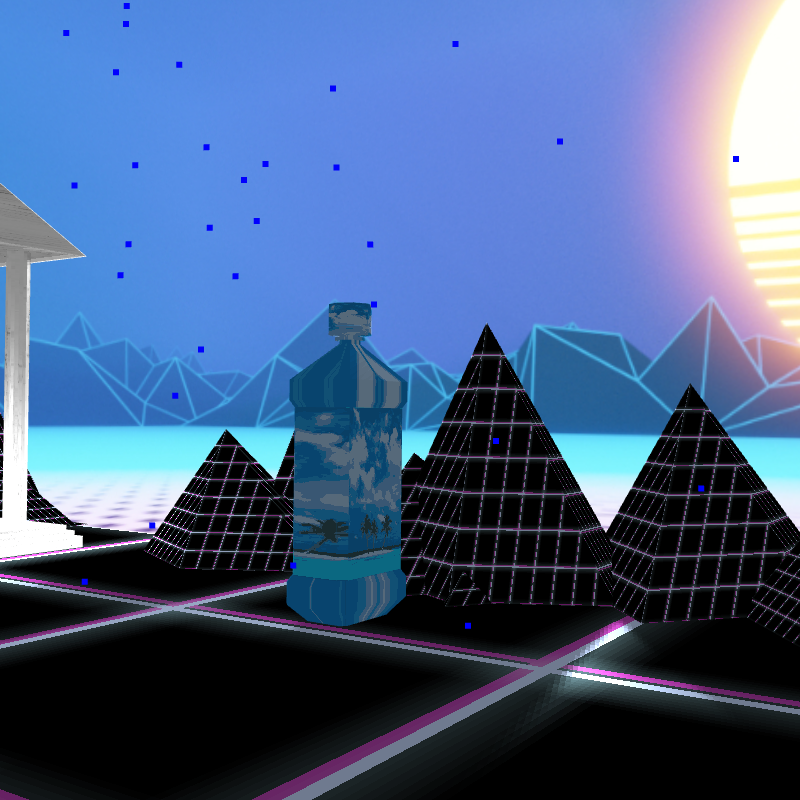
\includegraphics[width=0.3\textwidth]{large.png}
    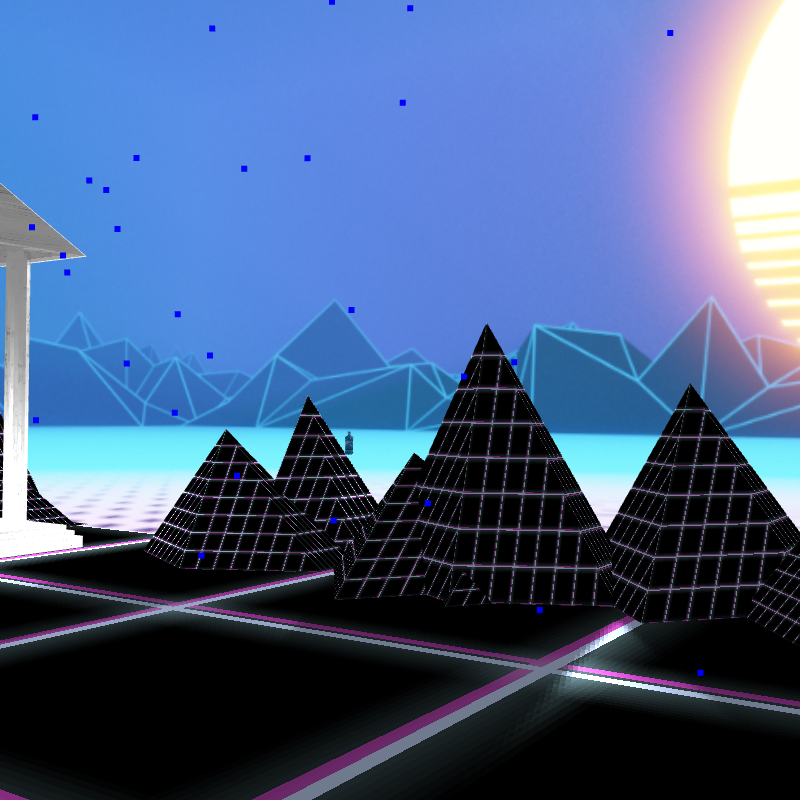
\includegraphics[width=0.3\textwidth]{small.png}
    
    The Fiji water bottle grows and shrinks in size.
\end{center}

\begin{center}
    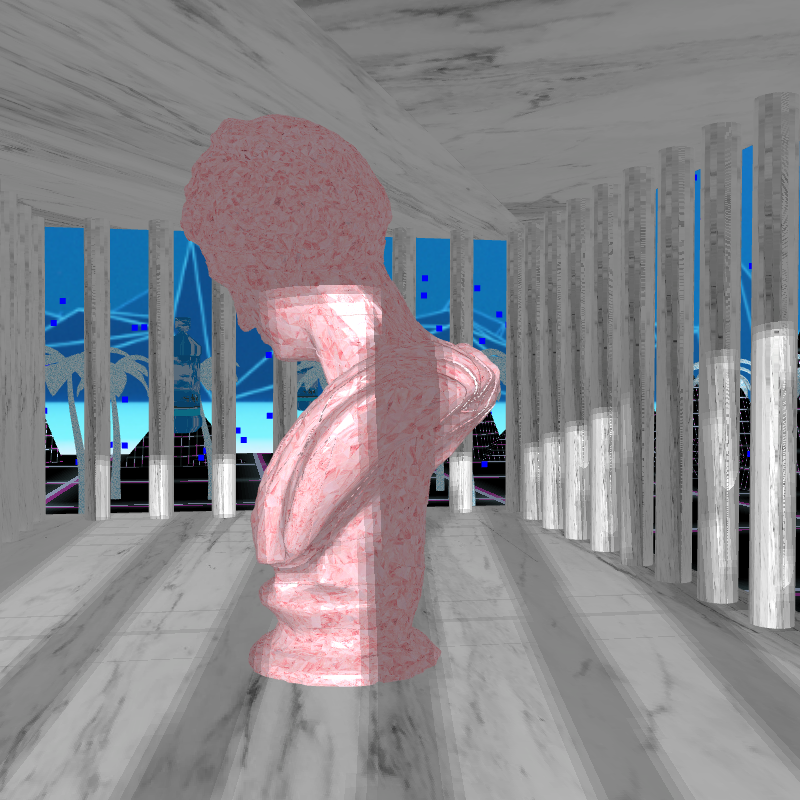
\includegraphics[width=0.3\textwidth]{statue1.png}
    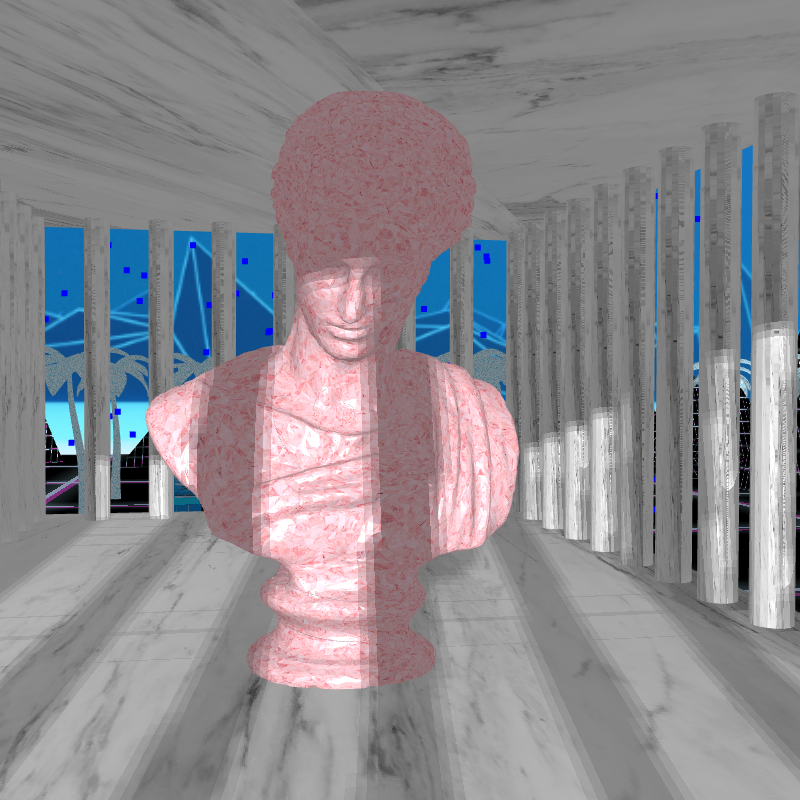
\includegraphics[width=0.3\textwidth]{statue2.png}
    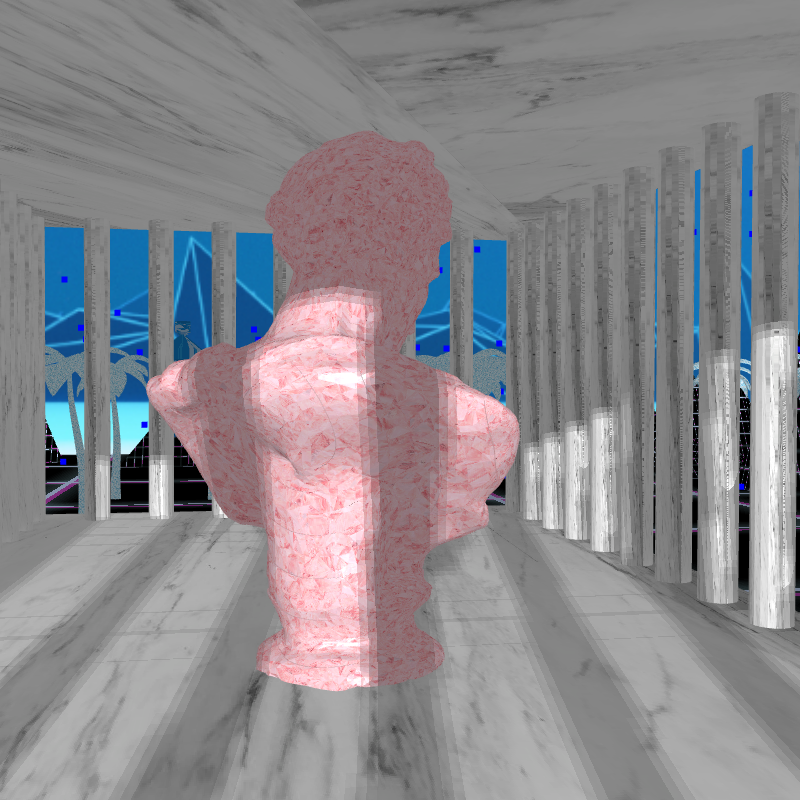
\includegraphics[width=0.3\textwidth]{statue3.png}
    
    The Statue spins in a circle.
\end{center}

\newpage
\section{Technical Details}

% Cameras
We have two cameras implemented in our project. The first camera is a flying camera that you can position anywhere, to implement this we implemented operations to move the camera's position and to pitch, yaw, and roll the camera. These operations update the eye, u, v, and n vectors. The camera calculates a camera matrix using the lookAt API and also provides a method to get the projection matrix (perspective). Our shaders use the camera and projection matrices to transform the world relative to the camera and projection. The second camera is a camera attached to the Tesla CyberTruck. This camera works differently in that the controls move the truck. The camera is always positioned at the truck's location but raised in the Y direction, and looking in the direction that the truck is pointed towards.

% Texture mapping
Texture mapping is done through the WebGL API for Texture2D; all textured 3D objects maintain an array of texture coordinates per each vertex to map the texture on. The skybox uses a texture cube map to texture each of the six sides of the skybox with a different image.

% Lighting
Lighting is done in the shader using per-fragment shading. We have implemented two lights, one is a directional light and the other is a spotlight. The spotlight is positioned at the same location as the Tesla CyberTruck and pointed in the direction of the truck, to simulate the truck's front lights. The spotlight does not use a dropoff factor with regard to Z distance as this made the effect of the spotlight hard to see. The spotlight fades out from the center of the light and there is a cutoff angle implemented.

% Animated objects
To animate objects, we implemented methods to transform the object's model matrix, such as translation, rotation, and scaling. The animated objects keep track of data regarding the current animated frame (such as rotation angle) and on draw, update these values and update the model matrix.

% Picking
Picking is done through raycasting. We have an input handler which runs every time the user clicks and tracks the mouse X and Y positions. These positions are converted into canvas positions, and then transformed into a ray coming from the center of the camera towards the position on the canvas that the user clicked on. We run this ray through every drawable object and calculate whether the ray hits the object, and if so, solve for the time ($t$) at which the ray hits the object. If a ray hits an object multiple times, we select the smallest time $t$ as the time of hit. Then, going through all objects, we look and see if any object is hit. If so, we select the object associated with the smallest time $t$ (so that we do not select some object behind the picked object). We then call the onPick handler method to let the object know it was picked. This usually results in some Boolean being set, which then updates the object's animation in the object's draw method.

% Dynamically generated objects
We have two types of dynamically generated objects - randomly generated objects, and objects that can be created on command. The randomly generated objects include things such as palm trees, Fiji water bottles, and mountains. The palm trees and water bottles are created with random X and Z coordinates and initial rotations. The mountains are randomly placed along the edges of the plane and the heights of the mountains are random. For objects that can be created on command, the dolphins can be created with a keypress. On pressing the key to create a dolphin, a dolphin is randomly placed somewhere near the edge of the plane and added to the list of drawable objects. This dolphin is animated to jump to the other edge of the plane. When the dolphin reaches the other edge, it sets a Boolean in its draw method letting the program know that it can be deleted. The main draw loop goes through all objects and removes any that can be safely deleted. So these dynamic objects support creation and deletion from the scene.

% New object geometry (cylinders/parthenon/OBJ)
We implemented two types of new object geometry. The first new geometry is 3D models that are loaded with an OBJ loader module. To build this module, we extended the SMF model from a prior homework to support more commands. In addition to vertices and faces, the OBJ format also has commands for vertex normals (vn) and vertex textures (vt). These commands allow us to support lighting and texturing with the models. The face command (f) is significantly different, though, as this command can specify three or more vertex groupings, each grouping listing at least vertices, with vertex normals and vertex textures being optional. We had to change the parser significantly to support these changes. If more than three vertices are supplied, we essentially treat the list of vertices as a triangle fan when building the face. The normals and textures are used as provided. If no normals are provided in the command, we compute the normal using the cross product of the vertices. If no textures are provided in the command, we assign default texture coordinates to the vertices. We did not implement all OBJ commands (we do not have support for .mtl files, for instance) as we were limited due to time constraints, but did implement all commands necessary so that we could import OBJ models that support lighting and texture mapping. The second new object geometry is a parthenon that we made by hand. To build this, we created a new cylinder object and instantiate multiple cylinders as the pillars of the parthenon. We took the pyramid class from a previous homework and adjusted the topmost vertices to make it a roof. The base of the parthenon is made up of layered transformed cubes. The statue inside the parthenon is created with the OBJ loader module.

% Reflection

Reflection is done as suggested in class through environment mapping. The CyberTruck has reflection through an environment map that is generated for it. At the location of the truck, we position a new camera class and direct it towards each of the six directions to render the scene (minus the truck) to a framebuffer. The buffer then writes these renderings out to textures of a cube map. We then compute the reflection vector relative to the current camera and use that to find the part of the cube map that should be drawn on each fragment of the truck. What we achieve is a very nice looking reflection effect on the truck that changes as you drive the truck around the map.

% Shadows

Shadows are done through a multi-pass render, using the Z-buffer algorithm as suggested in class. We position a camera at the location of our direction light and render a modified version of the scene, where the shader computes the color purely based on the depth in the Z-direction. This scene is drawn to a 2D texture. We then render the scene again from the position of the directional light, and compare the depth of each vertex against the pixel that it gets mapped to in the 2D texture. If we find that the vertex is obscured (the depth is worse than the depth in the 2D texture), we multiply the lighting effect by a factor of 0.5, to achieve a shadow effect. We also compare the computed shadows in a 3x3 window around the current vertex and average them to apply a blurring effect to the edges of the shadow, so that the lower resolution of the 2D texture is not as evident.

% Particle Systems
Particle systems are rendering by drawing each particle as a point in WebGL. The particles are initialized with random velocities and positions, and a separate particle shader is used. We set up our particles to specifically move in the negative Y direction to simulate rain. Elements like flocking are implemented but go unused for this simulation. When a particle is considered to have hit either the plane or the Parthenon (done through checking the particle coordinates for a collision), we move the particle back to a Y-level of 10. We also update the gravity of the particles every time they are drawn; each particle has a random mass and the velocity increases by a fraction of the mass each time it is drawn. This results in an effective where the simulated rain gets more intense over time, like how rain might get worse in the middle of a storm.

% Custom shader

Additionally we implemented a custom shader filter for the truck. When the truck camera is enabled, we turn on a final filter at the end of the fragment shader. This filter generates an oil texture based upon the object's current time value and the position of the fragment relative to the campus. The oil texture interpolates a sine wave function for the color and is animated by the time; the time value is incremented per each draw iteration by every object, which slightly changes the sine function. We also have a CRT gridline filter which is done through mixing two sine waves over the X and Y axes which vary by intensity in both direction with the fragment color.

\newpage
\section{Work Allocation}

The work was allocated between the two authors as follows:
\begin{itemize}
    \item Stephen Hansen
    \begin{itemize}
        \item Cameras
        \item Texture mapping
        \item Lighting
        \item Animated objects
        \item Picking
        \item Dynamically generated objects
        \item OBJ loader and 3D models
        \item Reflection
        \item Shader filters
    \end{itemize}
    \item Kevin Karnani
    \begin{itemize}
        \item Texture mapping
        \item New object geometry (Parthenon)
        \item OBJ loader and 3D models
        \item Shadows
        \item Particle systems
        \item Shader filters
    \end{itemize}
\end{itemize}

\newpage
\section{Citations}

The textures used came from the following sources:
\begin{itemize}
\item \textbf{Vaporwave skybox} \url{https://vesta.janusxr.org/spyduck/synthwave-skybox-template}
\item \textbf{Crystal} \url{https://www.freepik.com/free-photos-vectors/crystal-texture}
\item \textbf{Fiji Water} \url{https://sketchfab.com/3d-models/fiji-water-bottle-219204daeb2f446ebbc3837df97e0a8a}
\item \textbf{Marble} \url{https://unsplash.com/s/photos/marble-texture}
\item \textbf{Pink marble} \url{https://fineartamerica.com/featured/pink-marble-texture-background-prairat-fhunta.html}
\item \textbf{Grid} \url{https://opengameart.org/content/vaporwave-grid}
\item \textbf{Water} \url{https://unsplash.com/s/photos/water-texture}
\end{itemize}

\noindent
The .OBJ files used came from the following sources:
\begin{itemize}
\item \textbf{Dolphin} \url{https://free3d.com/3d-model/-dolphin-v1--12175.html}
\item \textbf{Fiji Water} \url{https://sketchfab.com/3d-models/fiji-water-bottle-219204daeb2f446ebbc3837df97e0a8a}
\item \textbf{Tesla CyberTruck} \url{https://free3d.com/3d-model/tesla-cyber-truck-973749.html}
\item \textbf{Statue} \url{https://sketchfab.com/3d-models/glitch-bust-fc304fa242504070b69061abe99dbff0}
\item \textbf{Palm Trees} \url{https://www.turbosquid.com/3d-models/blender-carrot-crystal-oak-tree-3d-model-1189852}
\end{itemize}

%%% End document
\end{document}